\section{Conclusion}
\label{section:conclusion}
Further on this thesis will be closed with a conclusion.
Therefore, the research question: \enquote{\textit{Are Android smartphones suitable of working with \gls{see}?}} will be in focus one last time.
The research question can be interpreted into several sub questions. 
\begin{itemize}
    \item Is it possible to use \gls{see} on \gls{android} devices?
    \begin{itemize}
        \item Yes it is possible with the given implementation from chapter \ref{section:implementation}.
        The given implementation however is only a first approach and does not cover every functionality from the desktop version.
        Functions like reviewing source code are not implemented yet and need further solutions. 
    \end{itemize}
    \item Is it possible to run \gls{see} on any given \gls{android} device?
    \begin{itemize}
        \item No it is not as the results of chapter \ref{section:evaluation} show. 
        Two of the 20 participants could not attend the user study because the mobile version of \gls{see} crashed on their devices.
        18 of 20 participants however were able to use \gls{android}. 
        Five of these 18 participants reported performance issues.
        The bad performance of a device could have caused a worse result as discussed in section \ref{sec:experinece}.
        In summary, that means, in the current state of \gls{see}, an \gls{android} device with solid hardware is needed for a carefree use.
    \end{itemize}
    \item Does it make sense to use the mobile version or is the \gls{usability} too low? 
    \begin{itemize}
        \item The results discussed in section \ref{sec:usability} show that the \gls{sus}-score of the mobile version is significantly lower than the one of the desktop version.
        However, this does not have to mean that mobile version is not useful. 
        \cite{doi:10.1080/10447310802205776} provided a scale to rate the value of a \gls{sus}-score (see figure \ref{fig:sus_scale}).
        Accordingly, to Banger at al. a \gls{sus}-score below 50 means almost certainly that the product will have issues regarding \gls{usability}.
        On the other side a score between 70 and 90 is promising that the product will have a high acceptability.
        The \gls{sus}-score of the mobile version is therefore in the acceptable range even though it is significantly lower than the desktop versions score.
        It can probably be said that the mobile version is useful to have even though there is potential for improvement.
    \end{itemize}
\end{itemize}

\begin{figure}[htb]
    \centering
    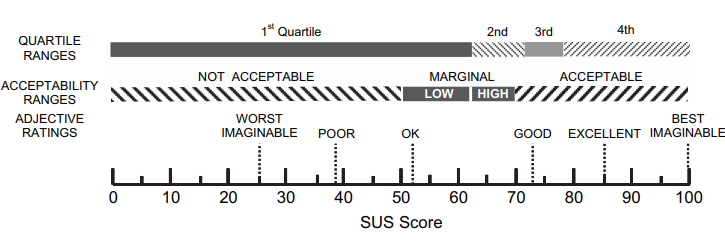
\includegraphics[width=1\textwidth]{Conclusion/img/sus.png}
    \caption{A comparison of mean System Usability Scale (SUS) scores by quartile,
    adjective ratings, and the acceptability of the overall SUS score by \cite{doi:10.1080/10447310802205776}}\label{fig:sus_scale}
  \end{figure}

  All in all the research question can be answered with \enquote{yes}.
  Regardless of the facts that the subjects needed significantly less time to solve the tasks in the user study with the desktop, the mobile version still seems to be acceptable and therefore suitable to be used.
  This can be additionally substantiated with the results from the \gls{ASQ} questionnaires, which just slightly differed between the two version.
  Also, as mentioned earlier, the \gls{sus}-score, even if significantly lower, seems to be in an acceptable range.

\subsection{Further Study and Ideas}
AR - \cite{santos2016guidelines}

\subsection{Closing Words}